\documentclass[11pt,a4paper]{article}
\usepackage{ifpdf}
\usepackage[utf8]{inputenc}
\usepackage[francais]{babel}
\usepackage[french]{varioref} 
\usepackage[pdftex]{graphicx}
\usepackage{listings}
\usepackage{color}
\usepackage{amssymb}
\usepackage{amsmath}

%\usepackage{floatflt}
\usepackage{lscape} %afficher une partie en paysage


%%% Pour du code source %%%%
 \definecolor{colKeys}{rgb}{0.5,0,0.33} 
 \definecolor{colIdentifier}{rgb}{0.16,0,1} 
 \definecolor{colComments}{rgb}{0.25,0.5,0.37} 
 \definecolor{colString}{rgb}{0.6,0.1,0.1} 
 \definecolor{shadow}{rgb}{0.5,0.5,0.5} 
 
 \lstset{ 
 basicstyle=\ttfamily\small,
 identifierstyle=\color{colIdentifier},
 keywordstyle=\color{colKeys},
 stringstyle=\color{colString},
 commentstyle=\color{colComments}
 }
 \lstset{language=python}



\begin{document}

%\tableofcontents
\thispagestyle{empty}
\begin{center}
\begin{tabular}{lr}
\begin{minipage}[l]{0.4\textwidth}
\begin{flushleft}

\includegraphics[scale=0.2]{logo.png}
\end{flushleft}
\end{minipage}
&
\begin{minipage}[r]{0.4\textwidth}
\begin{flushright}
\begin{tabular}{l}
Van De Walle Bernard  (A)\\
Francois Thibault (B) \\
Van Der Essen Frédéric (C)
\end{tabular}
\end{flushright}
\end{minipage}
\end{tabular}
\end{center}

\vspace{6.5cm}

\begin{center}
\textsc{INGI2132: Langages et traducteurs}
\end{center}

\bigskip

\begin{center}
{\Huge Rapport Final}
\end{center}

\vspace{7.5cm}
\begin{center}
		\textbf{Prof.} B. Le Charlier\\
\end{center}

\vspace{1.5cm}

\newpage

\begin{figure}[h!]
\begin{center}
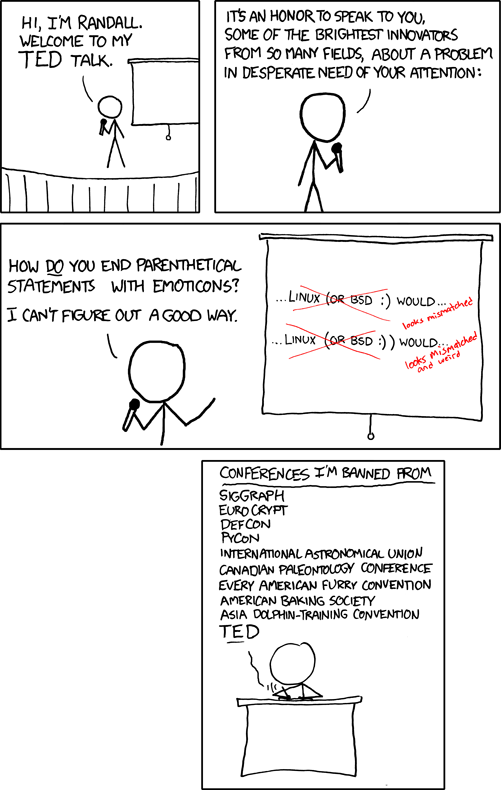
\includegraphics[scale=0.65]{xkcd.png}
\end{center}
\end{figure}
It is now possible with the HAPPY-) programming language !
\newpage

\section*{Introduction}
\section*{Syntaxe concrètes}

Notre langage s'inspire fortement du lisp, langage qui nous attirait par sa simplicité
et son élégance. Toutes les structures sont constituées de liste d'élément séparés par
des espaces, clos par des parenthèses. 

La syntaxe BNF suivante aurait pu être nettement plus simple, cependant nous avons choisi
de rendre explicites certains éléments de la syntaxe. Ainsi nous différentions le Nom ( <name> )
de la fonction de ses arguments, même si dans certains cas ce sont des entités syntaxiques identiques. 

Les appels de fonction sont de forme \emph{(Nom arg1 arg2 ...)}. A chaque opérateur du langage 
correspond une fonction, par exemple \emph{(+ 1 2)} Cependant nous avons donné un statut spécial
de <builtin\_call> à celles-ci afin d'empècher l'utilisateur de les redéfinir, et l'on espère,
de simplifier l'implémentation du futur interpréteur en lui permettant de repérer directement
les fonctions internes. 

Read et write sont eux aussi implémentés en tant que fonction, la fonction write renvoyant
l'argument donné en plus de l'imprimer sur la sortie standard, permettant de les intégrer
à des expressions normales. 

Cette syntaxe a l'avantage d'avoir peu de caractères réservés $\{ (,),.,[,]\}$, et peu
de restrictions sur les identifiants (ceux ci ne peuvent commencer par un chiffre). Il
est donc facile de créer de nouveaux opérateurs, parfois amusant comme des smileys , ce
qui a donné le nom de notre langage.  

Notre langage différe cependant du lisp dans le fait qu'il n'est pas composé d'une seule
expression, mais d'une suite de fonctions et méthodes, et que celles-ci sont composées de
liste d'instructions. Ainsi l'assignation et les conditionnelles ne sont pas des expressions.
Le langage ainsi défini est donc impératif.

Les objets sont implémentés comme des listes de longueur fixe qui peuvent être crées dynamiquement
grâce à la fonction new.

Les commentaires sont entre brackets et leur contenu est remplacé par un espace par l'analyseur lexical. 

L'ensemble des caractères acceptables par le programme est constitué d'un sous-ensemble de l'ASCII,
constitué de l'union de <caracter> et de <reserved\_caracter>. Les caractères Tab et NewLine sont aussi
reconnu mais leur valeur peut dépendre de la plateforme. 

\subsection{Syntaxe initiale}
Voici la syntaxe en notation BNF.
\begin{verbatim}
<Reserved_words>    ::= set | if | while | write | fun | method 
      | null | true | false | read | this 
<bin_id> ::=  + | - | * | / | % | '|' | & | < | > | <= | >=
<un_id>  ::=  ! | neg | new
<Reserved_caracter> ::=  ( | ) | . | [ | ]
<digit> ::= 0..9 
<pnumber> ::=  <digit> | <number> <digit> 
<number>  ::= - <pnumber> | <pnumber>
<caracter> ::= a..z | A..Z | ! | @ | # | $ | % | ^ | & | * 
		| { | } '|' | | _ | , | ? | - | + | = | / 
		| \\ | > | < | : | ; | ~ | \ | " 
<sp> ::= lambda |   | NewLine | Tab | <sp> <sp>
<esp> ::=   <sp>
<Id> ::= <caracter> | <Id> <caracter> | <Id> <digit>   
<meth_or_fun> ::= <methode> | <function>
<program> ::=  <meth_or_fun> | <program> <sp>  <meth_or_fun> 
<function> ::= (<sp> fun <sp> ( <sp> <Name> <esp> <arglist> <sp>) 
		<sp> <instr_list> <sp>) 
<arglist> ::= <Id> | <Id> <esp> <arglist>
<methode> ::= (<sp> method . <Number> <sp> 
	      ( <sp> <Name> <esp> <arglist> <sp> ) <instr_list>  <sp> )
<instr_list> ::= <instr> | ( <sp> <instr_list_np> <sp> ) 
<instr_list_np> ::= <instr> | <instr> <esp> <instr_list_np>
<instr> ::= <conditional> | <while_block> | <call> 
			  | ( <sp> return <esp> <expr> <sp> ) 
			  | (<sp> skip <sp>)
<conditional> ::= (<sp> if <esp> <expr> <esp> <instr_list>
		  <esp> <instr_list> <sp> ) 
<while_block ::= ( <sp> while <esp> <expr> <esp> <instr_list> <sp> ) 
<call> ::= <function_call> | <method_call> | <builtin_call> 
<builtin_call> ::= <assignment> | <read_call> | <write_call> | <arithmetic>
<assignment> ::= ( <sp> set <esp> <left_Id> <esp> <expr> <sp> ) 
<read_call>  ::= ( <sp> read <sp> ) 
<write_call> ::= ( <sp> write <esp> <expr> )
<arithmetic> ::= <binary> | <unary>
<binary ::= ( <sp> <bin_id> <esp> <expr> <esp> <expr> <sp> )
<unary>  ::=  ( <sp> <un_id> <esp> <expr> <sp> ) | return | skip
<left_Id> ::= <Id> | <Id> . <expr> | this . <expr>
<function_call>  ::= ( <sp> <Id> <esp> <expr_list_np> <sp> )
<expr_list_np> ::= lambda | <expr> | <expr> <esp> <expr_list_np>
<method_call>  ::= ( <sp> <method_id> <esp> <expr_list_np> <sp> )
<method_id>    ::= <Id> . <Id> | super . <Id> 
<expr>         ::= <call> | <left_Id> | <number> | null | true | false | this  
\end{verbatim}

\subsection{Syntaxe de l'analyseur Lexical}

Notre analyseur lexical nous permet de parser notre programme et d'en ressortir une liste de jetons ordonnés concret. 
La syntaxe qui sera analysée ne sera bien évidemment pas aussi fine que la syntaxe de base définie dans la section précedente 
( en effet, quel serait l'objectif de ressortir des jetons contenant chacun un et un seul caractère ! ). 
Les jetons contiendront donc des unités concrètes tel que les identifieurs, les nombes, les nombres négatifs, les parenthèse, etc etc..

Voici donc la syntaxe interpretée par l'analyseur syntaxique :

\subsection{Syntaxe initiale}
Nous avons définit un premier lieu cette syntaxe : 

\begin{verbatim}
<Reserved_words>    ::= set | if | while | write | fun | method 
      | null | true | false | read | new | + | - | * | / 
      | % | '|' | & | ! | < | > | <= | >= | neg | this 
      | return | skip
<meth_or_fun> ::= <method> | <function>
<Program> ::=  <meth_or_fun> | <Program>  <meth_or_fun>
<function> ::= (fun ( Id <arglist> ) <instr_list> ) 
<arglist> ::= Id | Id <arglist>
<methode> ::= (method ( Number ) (Id <arglist> ) <instr_list> )
<instr_list> ::= <instr> | ( <instr_list_np> ) 
<instr_list_np> ::= <instr> | <instr> <instr_list_np>
<instr> ::= <conditional> | <while_block> | <call> 
			  | ( return <expr> ) 
			  | ( skip )
<conditional> ::= (if <expr> <instr_list> <instr_list> ) 
<while_block ::= ( while <expr> <instr_list>) 
<call> ::= <function_call> | <method_call> | <builtin_call> 
<builtin_call> ::= <assignment> | <read_call> | <write_call> | <arithmetic>
<assignment> ::= ( set <left_Id> <expr> ) 
<read_call>  ::= ( read ) 
<write_call> ::= ( write <expr> )
<arithmetic> ::= <binary> | <unary>
<binary ::= (<bin_id> <expr> <expr>)
<bin_id> ::=  + | - | * | / | % | '|' | & | < | > | <= | >=
<unary>  ::=  (<un_id> <expr>)
<un_id>  ::=  ! | neg | new
<left_Id> ::= Id | Id . <expr> | this .  <expr>
<user_call>  ::= ( <Id> <expr_list_np> )
<expr_list_np> ::= lambda | <expr> | <expr> <expr_list_np>
<method_call>  ::= ( <method_id> <expr_list_np>)
<method_id> ::= <Id> . <Id> | super . <Id> 
<expr> ::= <call> | <left_Id> | <number> | null | true | false | this  
\end{verbatim}


\subsection{Syntaxe WP de l'analyseur grammatical}

\section{Exemple de programmation HAPPY}


\subsection{Example1}
Un programme complet. 
\begin{verbatim}
(fun (:-D) (write 42))
(fun (** a b) (
	(set cpt b)
	(set res 0)
	(while (> cpt 0) 
		(
			(set r (* res b))
			(set cpt (- cpt 1))	
		)
	)
	(return R)
))
(fun (main) (
	(HelloWorld)
	(set B (** 4 2))
	(return (write B))
))

(method (4) (-> level) (return this.level))

\end{verbatim}
Exemple de code intéressant. 
\begin{verbatim}

(method.2 (next) (return this.1))
(method.2 (val)  (return this.2))
	[Creation d'un noeud de linked list]
(fun (N x) ((set n (new 2)) (set n.2 x) (set n.1 null) (return n)) )
	[Ajoute un noeud a une linked list] 
(fun (-> Node NextNode) ( (set Node.1 NextNode) (return Node)) )

(fun (main) (
	(set A (->(N 1) (->(N 2) (->(N 3) (N 4)))))
	(while A (
		(write (A.val))
		(set A (A.next))
	))
	(return 0)
))
\end{verbatim}

\subsection{Exemple2}

Voici un exemple de programmation Happy :

\begin{verbatim}

(fun (Adder A B)(
	(set C (+ A B))
	(return C)
)

(fun (exposant A B)(
	(set result A)
	(set I 0)
	(while (I<B) 
		(set result (* result A))
		(set I (+ I 1))
	)
	(return result)
	)
)

(method(3) (Moore A B)(
	(return (A*B*1.5))
	)
)

(fun (main) (
	(set A 5)
	(set B 10)
	(set C (Adder A B))
	(set D (Exposant C B))
	(write (moore A B))
	)
)

\end{verbatim}

Dans cet exemple on montre différente manière de traiter des nombres grâce à des opérations relativement simple, tel que l'addition et l'exposant. Cet exemple permet d'illustrer la syntaxe de manière concrète.



\section{L'analyseur Lexical}

L'analyseur Lexical a pour fonction de sortir une suite de jeton concrêt et de assez haut niveau, permettant de simplifier la tache du vérificateur de grammaire. Plus concrètement, il s'agit dans un premier temps de transformer un fichier texte en une suite de caractère, et de les parser les un après les autres. Chaque caractère donnera lieu à une action précise, par exemple les caractères spéciaux tel que les paranthèse et les points, etc... donnent lieux à un jeton entier.
Les caractères qui ne sont pas des caractères spéciaux vont quand à eux remplir un buffer , qui sera rempli des qu'un caractère spécial ou délimiteur sera rencontré. Une fois qu'un caractère de ce type est rencontré, on procédera à l'analyse de ce que contient le buffer, et selon le cas on en déterminera le type du jeton à donner.

La sortie de l'analyseur lexical sera donc une linkedlist contenant les jetons dans l'ordre correspondant au programme.

Voici la spécification de la méthode principale qui permet d'obtenir la linkedlist de jetons :
{\tiny
\begin{verbatim}
	/**
	 * @pre Le parser est initialisé avec le programme.
	 * @post Le programme est transformé en un tableaux de caractère, 
et est analysé caractère par caractère, permettant de créer 
une suite logique de jetons.
	 * @return La linkedList contenant tout les tokens.
	 * @throws LexicalError
	 */
\end{verbatim}
}
\section{Test Analyseur Lexical}

Voici quelques tests qui permettent d'illustrer le comportement de l'analyseur lexical .Afin de visualiser la sortie de l'analyseur , on sort le type et le nom du jeton à la sortie standard (stdin).

\subsubsection{Test qui marche}
Voici le programme que l'analyseur lexical doit prendre en entrée pour ce premier test :
\begin{verbatim}
(fun (test A B C)((return (+ A(+ B C)))))
\end{verbatim}
Voici ce qu'on obtient en sortie :
{\tiny
\begin{verbatim}
token 0 : (	(
token 1 :  	esp
token 2 : fun	fun
token 3 :  	esp
token 4 : (	(
token 5 :  	esp
token 6 : test	id
token 7 :  	esp
token 8 : A	id
token 9 :  	esp
token 10 : B	id
token 11 :  	esp
token 12 : C	id
token 13 :  	esp
token 14 : )	)
token 15 :  	esp
token 16 : (	(
token 17 :  	esp
token 18 : (	(
token 19 :  	esp
token 20 : return	return
token 21 :  	esp
token 22 : (	(
token 23 :  	esp
token 24 : +	binary
token 25 :  	esp
token 26 : A	id
token 27 :  	esp
token 28 : (	(
token 29 :  	esp
token 30 : +	binary
token 31 :  	esp
token 32 : B	id
token 33 :  	esp
token 34 : C	id
token 35 :  	esp
token 36 : )	)
token 37 :  	esp
token 38 : )	)
token 39 :  	esp
token 40 : )	)
token 41 :  	esp
token 42 : )	)
token 43 :  	esp
token 44 : )	)
token 45 :  	esp
\end{verbatim}
}
L'analyseur lexical marche donc parfaitement , et permet de reconnaitre les différents type de token, ainsio que leurs valeurs.

\subsubsection{Test qui ne marche pas}

Voici un test qui ne marche pas :

(fun (azerty$\mu$ A B)((return 3) ))
Exception in thread "main" list.all.LexicalError: $\mu$


Ce Test ne marche pas car un caractère illégal a été utilisé, et en conséquence l'analyseur lexical le reconnait et l'interdit.

\subsection{Autre Test qui ne marche pas}

Voici un dernier test afin d'illustrer notre analyseur lexical : 

\begin{verbatim}
.(fun (test A B)((return 3) ))
Exception in thread "main" list.all.LexicalError: Erreur : No starting point
\end{verbatim}

Ce test illustre que Un programme ne peut pas démarrer par un point, et cela est bel et bien détecté et catché par notre analyseur lexical.



\section{Vérificateur de grammaire}
	\subsection{BNF Parser}
	Le point de départ du vérificateur de grammaire est le parser BNF. Ce parser permet d'avoir sous une forme utilisable que nous détaillerons 
plus loin, les règles contenue dans le fichier. Le loader charge le fichier et le lit ligne par ligne.

Loader
\begin{verbatim*}
	/**
	 * initialize the rules loader, the file should be a valid BNF File
	 * that mean every rules look like that
	 * nonTerminal ::= rules1 | rules2 | .. | rulesN
	 * nonTerminal should be written like that : <id>
	 * Terminal should be written like that : 'term'
	 * special caracter  ' \ could be in a terminal symbole precede by a \
	 * 
	 * exemple : 
	 * <E> ::= <T> 
	 * <E> ::= '\\' <T> 
	 * <E> ::= <T> '+' <E>
	 * <T> ::= <F>
	 * <T> ::= <F> '*' <T> 
	 * <F> ::= '\''
	 *  
	 * @param file the path of the file
	 * @throws FileNotFoundException
	 * @throws IOException
	 * 
	 * the rules can be extract with the method getRules()
	 */
\end{verbatim*}

Avec chaque ligne le loader instancie une rule qu'il place dans une liste. La classe rule parse la ligne et sépare d'un coté le nom et de l'autre
une orListe qui représente une liste de règles \textit{ou}. Chaque éléments de la orList est une catList c'est à dire une liste de \textit{Term} qui forme une règles.

	\subsection{Architecture}
	Le vérificateur de grammaire est implémenté comme une série de test
	statique correspondant aux conditions de Weak Priority.
	
	Tous ces tests prennent en paramètre la grammaire (une liste de "Rules")

	Un test global - \emph{CheckAll} - se charge de tester l'ensemble de ces tests.


	\subsection{Test de symbole vide (\emph{CheckLambda})}
		Ce test s'assure qu'aucune règle n'a de symbole vide (lambda).
		Ce test parcourt simplement l'arbre de la définition grammaire et
		vérifie l'absence de terminaux lambda.
	\subsection{Test de conflit de préférence (\emph{CheckPrecedence)}}
		Ce test vérifie qu'il n'y ait pas de conflit entre les précédence
		de symbole. Le seul conflit autorisé est entre $'<.'$ et $'=.'$ qui donne
		la relation de précédence $'<.='.$

		Pour faire cela, le test construit deux ensemble pour chaque non-terminal :
		First et Last. First(A) contient l'ensemble des terminaux et non terminaux 
		pouvant se trouver sur l'extrème gauche de A. Last(A) contient l'ensemble
		des terminaux et non terminaux pouvant se trouver sur l'extrème droide de A. 

		Pour calculer Tous les First on utilise l'algorithme suivant :
		\begin{enumerate}
			\item Pour tout non terminal A de la grammaire : On identifie les règles correspondantes.
			Pour chacune d'entre elles on identifie si elles commencent par un terminal, et si
			c'est le cas on les ajoute à First(A).
			\item Pour tout non terminal A de la grammaire : On identifie les règles correspondantes,
			Pour chacune d'entre elles, on identifie si elles commencent par un non terminal B.
			Si c'est le cas on ajoute B et First(B) à First(A). 
			\item on répète l'étape précédente tant que les First changent.
		\end{enumerate}
		L'algorithme pour trouver les Last est identique à ceci près qu'on examine les cotés droit des règles.
		
		Une fois que l'on a ces deux ensembles et que l'on sait qu'il n'y a pas de symboles vide dans
		la grammaire on  peut calculer la table de précedence, grace à l'algorithme suivant :
		\begin{enumerate}
			\item On initialise tous les éléments de la table à 'Nothing'
			\item On identifie toutes les parties droites, et pour chacune d'entre elles on identifie tous les
			symboles cotes à cotes XY.
			\item On ajoute X$.=$Y dans la table.
			\item Si X non terminal : Pour tout symbole s dans Last(X), Pour tout terminal t dans First(Y)
				on met s$.>$t dans la table. Si Y est non-terminal on met s$.>$Y dans la table.
			\item Si Y non terminal : Pour tout symbole s dans First(Y), on met X $<.$ s dans la table.
			\item Si à un moment on met une relation dans la table là ou précédemment il n'y avait pas 'Nothing',
				on a un conflit. Les conflits impliquant $<.$ , =. et $<.=$ sont résolus en insérant $<.=$ dans
				la table. Les autres conflits sont marqués en tant que conflits et reportés. 
			\item Si il y a des conflits non résolus dans la table alors le Test échoue, la grammaire n'est pas valide
			Weak Precedence.
		\end{enumerate}
	\subsection{Test de Suffixe}
		Ce test vérifie que les relations de suffixe sont respectées. C'est à dire :
		Pour tout couple de règles Z $->$ B, X $->$ AYB, où A représente une suite de symbole, Y un symbole unique,
		et B et une suite non vide symboles, on vérifie que !(Y .= X) , !(Y $<.$ X) et !(Y $<.=$ X).
		
		Pour ce faire nous utilisons la méthode suivante : 
		Pour chaque règle Z $->$ B, pour toute autre règle X $->$ Y on regarde si on peut matcher B comme suffixe de Y.
		Dans l'affirmative, on identifie le symbole juste avant le suffixe. Nous pouvons a ce moment vérifier la
		condition décrite expliquée précédemment. Si elle n'est pas vérifiée. le Test échoue, la grammaire n'est pas valide.
	\subsection{Spécifications des méthodes importantes}
{\small
\begin{verbatim}


 	/**
	 * 
	 * @param rules The rules list
	 * @param table The precedence table
	 * @return a list of tuple (triple) 
	 * that contains the two conflicting rules and 
	 * the suffix the cause the conflict
	 */
	public static List<RulesTuple> checkSuffix(List<Rule> rules, 
	Hashtable<Term,Hashtable<Term,String>> table) {
	
	/**
	 * Regarde si la grammaire n'a pas de conflits de précédence.
	 * Affiche la table des précédence à la sortie standard.
	 * @param grammar Une grammaire cohérente : 
	 * tous les non terminaux ont au moins une règle. 
	 * @return true si la grammaire est valide, false sinon.
	 */
	public static boolean checkPrecedence(List<Rule> grammar){
	
	/**
	 * Met une relation de précédence dans la table de précédence et
	 * résout les conflits. Affiche les détails de l'erreur à la sortie
	 * standard en cas de conflits. Si le conflit est entre <. ou <.= ou =. 
	 * celui ci est résolu en insérant un <.= 
	 * 
	 * @param table la table de précédence
	 * @param X	le premier Terme
	 * @param Y le second Terme
	 * @param rel la relation de précédence ( EQ,LE,GE,LEQ,ERROR,NOTHING)
	 * @param rule la règle d'ou provient X et Y.
	 * @return true si il n'y a pas de conflits, false sinon. 
	 */
	public static boolean tableSet(Hashtable<Term,Hashtable<Term,String>> 
	table, Term X, Term Y, String rel, Rule rule){
	
	/**
	 * Calcule l'ensemble First pour chaque Terme correspondant aux Termes
	 * pouvant se trouver à l'extrème gauche de celui ci. 
	 * @param grammar la grammaire
	 * @return une Hashtable qui fait correspondre à chaque Terme son set First.
	 */
	public static Hashtable<Term,Set<Term>> FirstSet(List<Rule> grammar){
	
	/**
	 * Calcule la table de précédence WP et si celle ci contient des conflits.
	 * En cas de conflits, ceux ci sont affichés à la sortie standard.
	 * @param grammar la grammaire
	 * @param table une Hashtable à deux dimensions dont l
	 * es clefs sont tous les couples
	 * 			de termes existant dans grammar. 
	 *  Tous les éléments de table sont initialisés
	 * 			à NOTHING.
	 * @return true si il n'y a pas de conflits dans la table, false sinon. 
	 */
	public static  boolean precTable(List<Rule> grammar, 
	Hashtable<Term,Hashtable<Term,String>> table){
	
	/**
	 * Vérifie que la liste ne contient pas d'expensions vides,
	 * en cherchant les termes 'lambda' dans tous les termes de toutes
	 * les règles. 
	 * @param grammar la grammaire
	 * @return  true si la grammaire ne contient pas de terme 'lambda',
	 * 			false sinon.
	 */
	public static boolean checkLambda(List<Rule> grammar){


\end{verbatim}
}

\section{Test du vérificateur}
Nous avons testé notre vérificateur de grammaire avec les grammaires fournie sur icampus 
pour finalement tester avec notre grammaire. Ici je ne montrerai que le test final pour notre grammaire. 

\subsection{Premier Test}
{\tiny
\begin{verbatim}
<A> ::= <A> 'a'
<A> ::= <B>
<B> ::= 'a'
<B> ::= <A> <B>

Check conflit suffix : 
----------------------------
A   A
<.
----------------------------
----------------------------
B   A
<=
----------------------------
conflit avec a:true
A ::= A:false a:true
B ::= a:true 

conflit avec B:false
B ::= A:false B:false
A ::= B:false 
\end{verbatim}
}

Validity grammar : false


Ce test concorde bien avec l'exmple donné
{\tiny
\begin{verbatim}
Grammaire non WP :
règle 1 : B --> a 
règle 2 : A --> A a
A <. B
Grammaire non WP :
règle 1 : A --> B 
règle 2 : B --> A B
A <. A

\end{verbatim}
}


\subsection{Second Test}:
{\tiny
\begin{verbatim}
<E> ::= <T> 
<E> ::= '+' <T> 
<E> ::= <E> '+' <T> 
<T> ::= <F> 
<T> ::= <T> '*' <F> 
<F> ::= 'x' 
<F> ::= '(' <E> ')' 
\end{verbatim}
}
C'est bien une grammaire WP :
{\tiny
\begin{verbatim}
Precedence Table
    |(   |)   |*   |+   |T   |E   |F   |x   |
     ========================================
(   | <. |    |    | <. | <. | <= | <. | <. |
     ----------------------------------------
)   |    | .> | .> | .> |    |    |    |    |
     ----------------------------------------
*   | <. |    |    |    |    |    | .= | <. |
     ----------------------------------------
+   | <. |    |    |    | <= |    | <. | <. |
     ----------------------------------------
T   |    | .> | .= | .> |    |    |    |    |
     ----------------------------------------
E   |    | .= |    | .= |    |    |    |    |
     ----------------------------------------
F   |    | .> | .> | .> |    |    |    |    |
     ----------------------------------------
x   |    | .> | .> | .> |    |    |    |    |
     ----------------------------------------

No conflicts in table
Validity precedence : true
Check conflit suffix : 
Validity grammar : true
\end{verbatim}
}

\subsection{Troisième Test}
Dernière grammaire qui est normalement fausse :
{\tiny
\begin{verbatim}
E --> T 
E --> + T 
E --> T + E 
T --> F 
T --> F * T 
F --> x 
F --> ( E ) 

Precedence Table
    |(   |)   |*   |+   |T   |E   |F   |x   |
     ========================================
(   | <. |    |    | <. | <. | .= | <. | <. |
     ----------------------------------------
)   |    | .> | .> | .> |    |    |    |    |
     ----------------------------------------
*   | <. |    |    |    | .= |    | <. | <. |
     ----------------------------------------
+   | <. |    |    | <. | <= | .= | <. | <. |
     ----------------------------------------
T   |    | .> |    | .= |    |    |    |    |
     ----------------------------------------
E   |    | .= |    |    |    |    |    |    |
     ----------------------------------------
F   |    | .> | .= | .> |    |    |    |    |
     ----------------------------------------
x   |    | .> | .> | .> |    |    |    |    |
     ----------------------------------------

No conflicts in table
Validity precedence : true
Check conflit suffix : 
----------------------------
E   +
.=
----------------------------
conflit avec T:false
E ::= +:true T:false
E ::= T:false 

Validity grammar : false
\end{verbatim}
}

\end{document}
